% inspired from http://www.latex-community.org/forum/viewtopic.php?f=9&t=22340
\documentclass{article}

\usepackage{tikz}
\usetikzlibrary{arrows}

\begin{document}

% Exemple de graphe
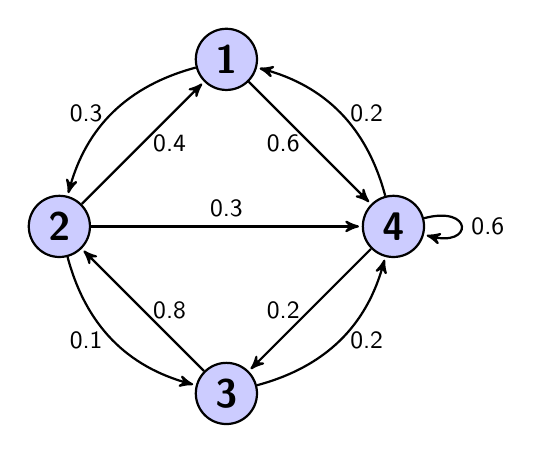
\begin{tikzpicture}[->, >=stealth', shorten >=1pt, auto, node distance = 3cm, thick, main node/.style = {circle, fill = blue!20, draw, font = \sffamily\Large\bfseries}]

	\node[main node] (1) {1};
	\node[main node] (2) [below left of = 1] {2};
	\node[main node] (3) [below right of = 2] {3};
	\node[main node] (4) [below right of = 1] {4};
	
	\path[every node/.style = {font = \sffamily\small}]
		(1) edge node [left] {0.6} (4)
			edge [bend right] node[left] {0.3} (2)
		(2) edge node [right] {0.4} (1)
			edge node {0.3} (4)
			edge [bend right] node[left] {0.1} (3)
		(3) edge node [right] {0.8} (2)
			edge [bend right] node[right] {0.2} (4)
		(4) edge node [left] {0.2} (3)
			edge [loop right] node {0.6} (4)
			edge [bend right] node[right] {0.2} (1);
\end{tikzpicture}

\vspace{2cm}
% Graphe orienté

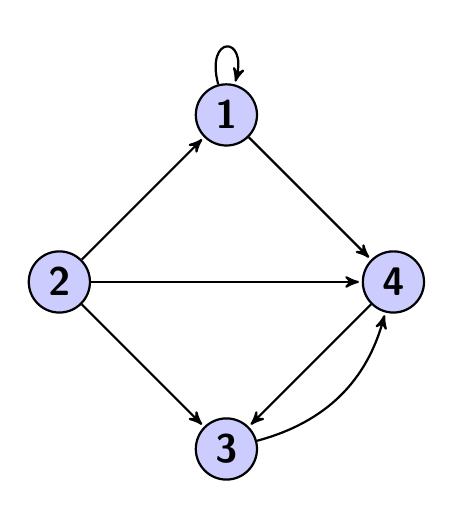
\begin{tikzpicture}[->, >=stealth', shorten >=1pt, auto, node distance = 3cm, thick, main node/.style = {circle, fill = blue!20, draw, font = \sffamily\Large\bfseries}]

	\node[main node] (1) {1};
	\node[main node] (2) [below left of = 1] {2};
	\node[main node] (3) [below right of = 2] {3};
	\node[main node] (4) [below right of = 1] {4};
	
	\path[every node/.style = {font = \sffamily\small}]
	(1) edge node [left] {} (4)
		edge [loop above] node {} (1)
	(2) edge node [right] {} (1)
		edge node {} (4)
		edge [right] node[left] {} (3)
	(3) edge [bend right] node[right] {} (4)
	(4) edge node [left] {} (3);
\end{tikzpicture}

\vspace{2cm}
% Graphe non orienté

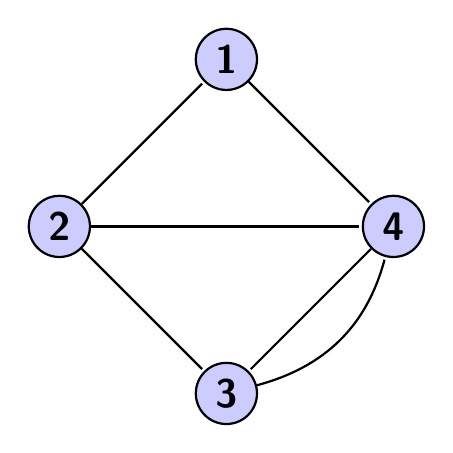
\begin{tikzpicture}[>=stealth', shorten >=1pt, auto, node distance = 3cm, thick, main node/.style = {circle, fill = blue!20, draw, font = \sffamily\Large\bfseries}]

	\node[main node] (1) {1};
	\node[main node] (2) [below left of = 1] {2};
	\node[main node] (3) [below right of = 2] {3};
	\node[main node] (4) [below right of = 1] {4};
	
	\path[every node/.style = {font = \sffamily\small}]
	(1) edge node [left] {} (4)
	(2) edge node [right] {} (1)
		edge node {} (4)
		edge [right] node[left] {} (3)
	(3) edge [bend right] node[right] {} (4)
	(4) edge node [left] {} (3);
\end{tikzpicture}

\vspace{2cm}
% Graphe pondéré (exemple de carte routière)

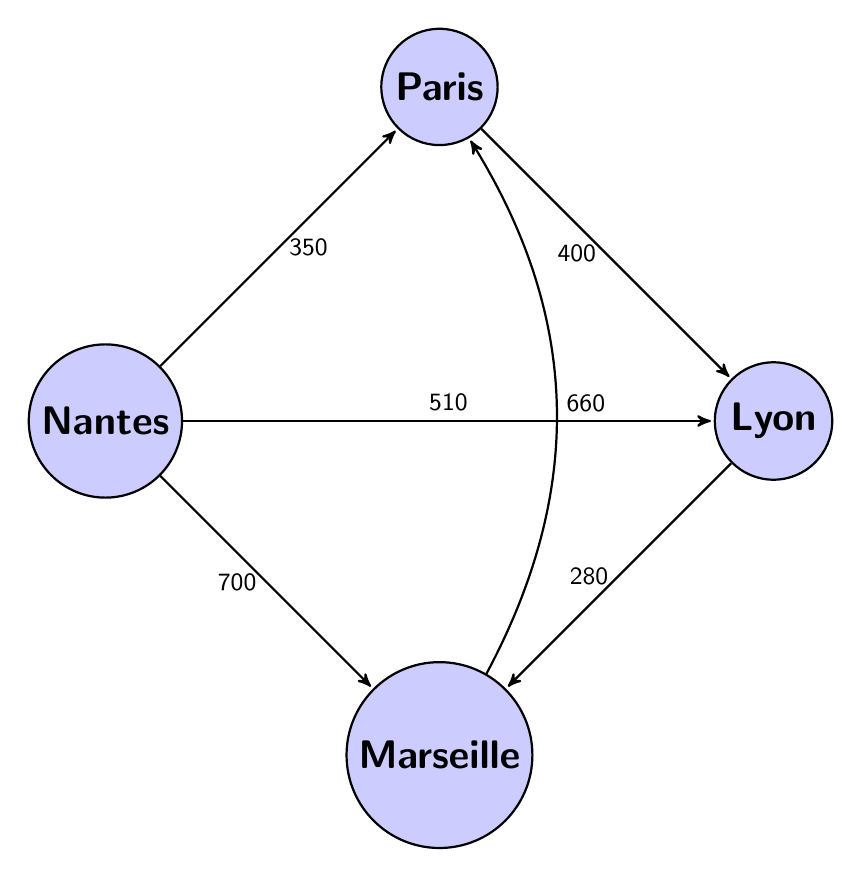
\begin{tikzpicture}[->, >=stealth', shorten >=1pt, auto, node distance = 6cm, thick,main node/.style = {circle, fill = blue!20, draw, font = \sffamily\Large\bfseries}]

	\node[main node] (1) {Paris};
	\node[main node] (2) [below left of = 1] {Nantes};
	\node[main node] (3) [below right of = 2] {Marseille};
	\node[main node] (4) [below right of = 1] {Lyon};
	
	\path[every node/.style = {font = \sffamily\small}]
	(1) edge node [left] {400} (4)
	(2) edge node [right] {350} (1)
		edge node {510} (4)
		edge [right] node[left] {700} (3)
	(3) edge [bend right] node[right] {660} (1)
	(4) edge node [left] {280} (3);
\end{tikzpicture}

\vspace{2cm}
% Graphe cyclique

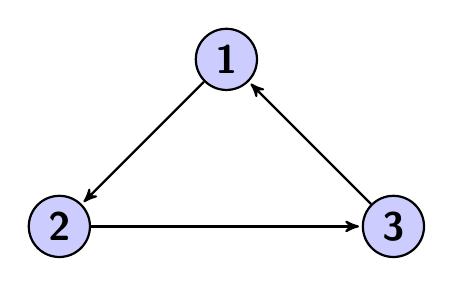
\begin{tikzpicture}[->, >=stealth', shorten >=1pt, auto, node distance = 3cm, thick, main node/.style = {circle, fill = blue!20, draw, font = \sffamily\Large\bfseries}]

	\node[main node] (1) {1};
	\node[main node] (2) [below left of = 1] {2};
	\node[main node] (3) [below right of = 1] {3};
	
	\path[every node/.style = {font = \sffamily\small}]
	(1) edge node [right] {} (2)
	(2) edge node {} (3)
	(3) edge node [left] {} (1);
\end{tikzpicture}

\vspace{2cm}
% Graphe acyclique

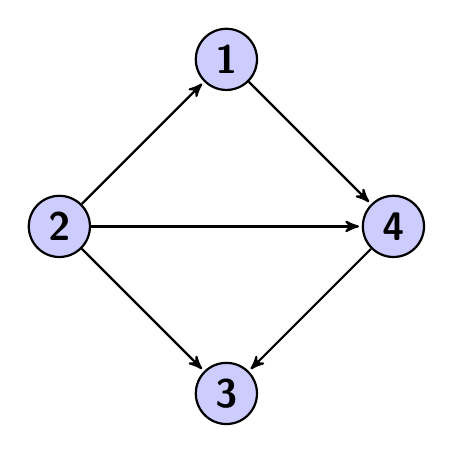
\begin{tikzpicture}[-> ,>=stealth', shorten >=1pt, auto, node distance = 3cm, thick, main node/.style = {circle, fill = blue!20, draw, font = \sffamily\Large\bfseries}]

	\node[main node] (1) {1};
	\node[main node] (2) [below left of = 1] {2};
	\node[main node] (3) [below right of = 2] {3};
	\node[main node] (4) [below right of = 1] {4};
	
	\path[every node/.style = {font = \sffamily\small}]
	(1) edge node [left] {} (4)
	(2) edge node [right] {} (1)
		edge node {} (4)
		edge [right] node[left] {} (3)
	(4) edge node [left] {} (3);
\end{tikzpicture}

\vspace{2cm}
% Graphe dense

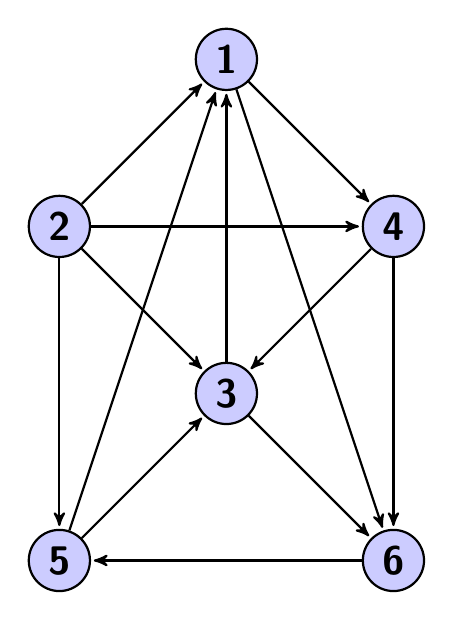
\begin{tikzpicture}[->, >=stealth', shorten >=1pt, auto, node distance = 3cm, thick, main node/.style = {circle, fill = blue!20, draw, font = \sffamily\Large\bfseries}]

	\node[main node] (1) {1};
	\node[main node] (2) [below left of = 1] {2};
	\node[main node] (3) [below right of = 2] {3};
	\node[main node] (4) [below right of = 1] {4};
	\node[main node] (5) [below left of = 3] {5};  
	\node[main node] (6) [below right of = 3] {6};
	
	\path[every node/.style = {font = \sffamily\small}]
	(1) edge node [left] {} (4)
		edge node [left] {} (6)
	(2) edge node [right] {} (1)
		edge node {} (4)
		edge [right] node[left] {} (3)
		edge node [right] {} (5)
	(3) edge node [right] {} (1)
		edge node [right] {} (6)
	(4) edge node [left] {} (3)
		edge node [right] {} (6)
	(5) edge node [right] {} (1)
		edge node [right] {} (3)
	(6) edge node [right] {} (5);
\end{tikzpicture}

\vspace{2cm}
% Graphe creux

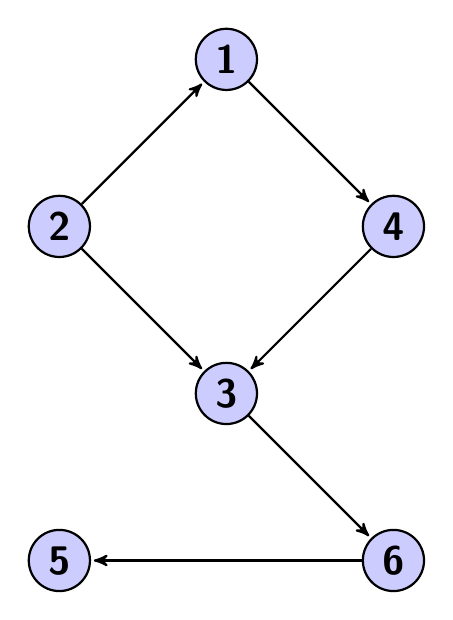
\begin{tikzpicture}[->, >=stealth', shorten >=1pt, auto, node distance = 3cm, thick, main node/.style = {circle, fill = blue!20, draw, font = \sffamily\Large\bfseries}]

	\node[main node] (1) {1};
	\node[main node] (2) [below left of = 1] {2};
	\node[main node] (3) [below right of = 2] {3};
	\node[main node] (4) [below right of = 1] {4};
	\node[main node] (5) [below left of = 3] {5};  
	\node[main node] (6) [below right of = 3] {6};
	
	\path[every node/.style = {font = \sffamily\small}]
	(1) edge node [left] {} (4)
	(2) edge node [right] {} (1)
		edge [right] node[left] {} (3)
	(3) edge node [right] {} (6)
	(4) edge node [left] {} (3)
	(6) edge node [right] {} (5);
\end{tikzpicture}

\vspace{2cm}
% Graphe connexe

	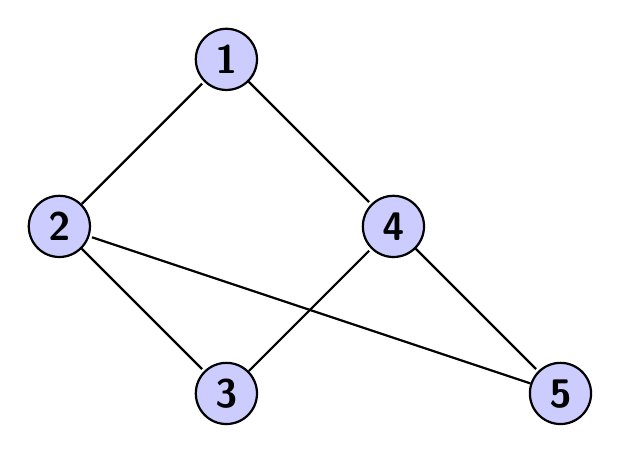
\begin{tikzpicture}[>=stealth', shorten >=1pt, auto, node distance = 3cm, thick, main node/.style = {circle, fill = blue!20, draw, font = \sffamily\Large\bfseries}]
	
	\node[main node] (1) {1};
	\node[main node] (2) [below left of = 1] {2};
	\node[main node] (3) [below right of = 2] {3};
	\node[main node] (4) [below right of = 1] {4};
	\node[main node] (5) [below right of = 4] {5};
	
	\path[every node/.style = {font = \sffamily\small}]
	(1) edge node [left] {} (4)
	(2) edge node [right] {} (1)
		edge [right] node[left] {} (3)
	(3) edge node[right] {} (4)
	(4) edge node[right] {} (5)
	(5) edge node [left] {} (2);
\end{tikzpicture}

\end{document}